\documentclass[tikz,border=0pt]{standalone}
\usetikzlibrary{calc}
% Palette: the 3D gym's colours (crates/core/src/mesh.rs, data/shaders/scene.frag).
\definecolor{sky}{HTML}{DCE6EE}
\definecolor{skyhi}{HTML}{F2F6F9}
\definecolor{wall}{HTML}{EDE6D3}
\definecolor{walldark}{HTML}{D6CCB4}
\definecolor{stripeblue}{HTML}{2F5CBF}
\definecolor{stripegold}{HTML}{F8C537}
\definecolor{window}{HTML}{CFE6FF}
\definecolor{windowlit}{HTML}{F6FBFF}
\definecolor{wood}{HTML}{DBA86B}
\definecolor{wooddark}{HTML}{B98549}
\definecolor{woodline}{HTML}{C9965A}
\definecolor{mat}{HTML}{2961CC}
\definecolor{matlit}{HTML}{4A82E8}
\definecolor{matdark}{HTML}{1C4597}
\definecolor{matseam}{HTML}{16377A}
\definecolor{red}{HTML}{DD3D38}
\definecolor{redlit}{HTML}{F06A5E}
\definecolor{reddark}{HTML}{A92A27}
\definecolor{yellow}{HTML}{F9C02E}
\definecolor{yellowlit}{HTML}{FFDB6B}
\definecolor{yellowdark}{HTML}{C9961C}
\definecolor{green}{HTML}{3FA866}
\definecolor{greenlit}{HTML}{62C98A}
\definecolor{greendark}{HTML}{2C7D4B}
\definecolor{pink}{HTML}{F27A93}
\definecolor{pinklit}{HTML}{F7A1B3}
\definecolor{orange}{HTML}{F28A2E}
\definecolor{orangelit}{HTML}{F7AE66}
\definecolor{orangedark}{HTML}{C2671A}
\definecolor{sky2}{HTML}{7FB8F0}
\definecolor{purple}{HTML}{8B5CC8}
\definecolor{skin}{HTML}{F2C49A}
\definecolor{skinlit}{HTML}{F8D8B8}
\definecolor{skindark}{HTML}{D9A47A}
\definecolor{skinb}{HTML}{B9835A}
\definecolor{skinbdark}{HTML}{93653F}
\definecolor{shirt}{HTML}{E2463F}
\definecolor{shirtdark}{HTML}{B23430}
\definecolor{shirtb}{HTML}{2F7DD8}
\definecolor{shirtbdark}{HTML}{225DA6}
\definecolor{shorts}{HTML}{21305A}
\definecolor{shortsdark}{HTML}{151F3D}
\definecolor{shoe}{HTML}{FFFFFF}
\definecolor{shoedark}{HTML}{D8DDE3}
\definecolor{hair}{HTML}{4A2F1C}
\definecolor{band}{HTML}{F8C537}
\definecolor{chick}{HTML}{FBE48F}
\definecolor{chicklit}{HTML}{FFF2BE}
\definecolor{chickdark}{HTML}{DCC064}
\definecolor{comb}{HTML}{E2302E}
\definecolor{beak}{HTML}{F28A2E}
\definecolor{noodle}{HTML}{57D163}
\definecolor{noodledark}{HTML}{3A9E45}
\definecolor{ball}{HTML}{D8302B}
\definecolor{balldark}{HTML}{A5211D}
\definecolor{balllit}{HTML}{F0645D}
\definecolor{duck}{HTML}{FFD12E}
\definecolor{duckdark}{HTML}{E0A814}
\definecolor{foam}{HTML}{2F6BE0}
\definecolor{foamdark}{HTML}{214FAD}
\definecolor{white}{HTML}{FFFFFF}
\definecolor{ink}{HTML}{1E2B45}
\definecolor{netline}{HTML}{9AA9BF}
\definecolor{glow}{HTML}{FFF4C2}
\begin{document}
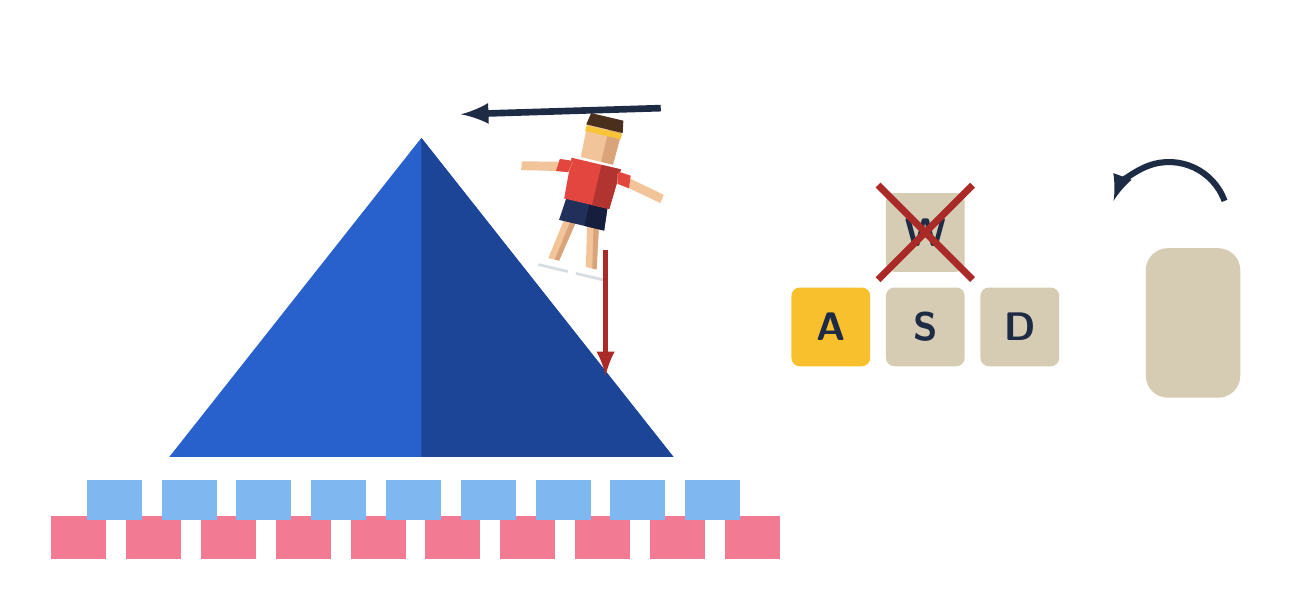
\begin{tikzpicture}[x=1cm,y=1cm]
\useasboundingbox (0,0) rectangle (16,7);
\fill[white] (0,0) rectangle (16,7);
% ---- the ramp, end-on: a ridge over a foam pit ----
\fill[mat] (1.8,1.55) -- (5,5.6) -- (8.2,1.55) -- cycle;
\fill[matdark] (5,5.6) -- (8.2,1.55) -- (5,1.55) -- cycle;
\foreach \i in {0,...,9} {\fill[pink] ({0.3+\i*0.95},0.25) rectangle ({1.0+\i*0.95},0.8);}
\foreach \i in {0,...,8} {\fill[sky2] ({0.75+\i*0.95},0.75) rectangle ({1.45+\i*0.95},1.25);}
\begin{scope}[shift={(6.89,3.878)},scale=0.7,rotate=-13.316]
\fill[shoe] (-0.6,0) -- (-0.05,0) -- (-0.05,0.16) -- (-0.55,0.2) -- cycle;
\fill[shoedark] (-0.6,0) -- (-0.05,0) -- (-0.05,0.05) -- (-0.6,0.05) -- cycle;
\fill[shoe] (0.1,0) -- (0.65,0) -- (0.65,0.16) -- (0.15,0.2) -- cycle;
\fill[shoedark] (0.1,0) -- (0.65,0) -- (0.65,0.05) -- (0.1,0.05) -- cycle;
\fill[skin] (-0.45,0.18) -- (-0.25,0.18) -- (-0.11,0.95) -- (-0.33,0.95) -- cycle;
\fill[skindark] (-0.33,0.18) -- (-0.25,0.18) -- (-0.11,0.95) -- (-0.21,0.95) -- cycle;
\fill[skin] (0.25,0.18) -- (0.45,0.18) -- (0.31,0.95) -- (0.09,0.95) -- cycle;
\fill[skindark] (0.37,0.18) -- (0.45,0.18) -- (0.31,0.95) -- (0.21,0.95) -- cycle;
\fill[shorts] (-0.42,0.9) -- (0.42,0.9) -- (0.38,1.35) -- (-0.38,1.35) -- cycle;
\fill[shortsdark] (0.05,0.9) -- (0.42,0.9) -- (0.38,1.35) -- (0.05,1.35) -- cycle;
\fill[shirt] (-0.42,1.3) -- (0.42,1.3) -- (0.46,2.05) -- (-0.46,2.05) -- cycle;
\fill[shirtdark] (0.1,1.3) -- (0.42,1.3) -- (0.46,2.05) -- (0.1,2.05) -- cycle;
\fill[skin] (-0.42,1.98) -- (-0.45,1.8) -- (-1.3,1.62) -- (-1.32,1.78) -- cycle;
\fill[shirt] (-0.42,2) -- (-0.46,1.78) -- (-0.68,1.75) -- (-0.66,1.98) -- cycle;
\fill[skin] (0.42,1.98) -- (0.45,1.8) -- (1.3,1.62) -- (1.32,1.78) -- cycle;
\fill[shirt] (0.42,2) -- (0.46,1.78) -- (0.68,1.75) -- (0.66,1.98) -- cycle;
\fill[skin] (-0.3,2.1) -- (0.3,2.1) -- (0.32,2.72) -- (-0.32,2.72) -- cycle;
\fill[skindark] (0.08,2.1) -- (0.3,2.1) -- (0.32,2.72) -- (0.08,2.72) -- cycle;
\fill[hair] (-0.34,2.7) -- (0.34,2.7) -- (0.3,2.92) -- (-0.3,2.92) -- cycle;
\fill[band] (-0.33,2.58) -- (0.33,2.58) -- (0.33,2.68) -- (-0.33,2.68) -- cycle;
\end{scope}
% ---- what to do: hold the key toward the ramp's top ----
\draw[-latex,ink,line width=2.4pt] (8.04,5.978) -- (5.5,5.9);
% gravity
\draw[-latex,reddark,line width=2pt] (7.34,4.178) -- (7.34,2.578);
% the keys: A lit, D dim, W crossed out
\fill[yellow,rounded corners=3pt] (9.7,2.7) rectangle (10.7,3.7);
\node[ink,font=\sffamily\bfseries\Large] at (10.2,3.2) {A};
\fill[walldark,rounded corners=3pt] (10.9,2.7) rectangle (11.9,3.7);
\node[ink,font=\sffamily\bfseries\Large] at (11.4,3.2) {S};
\fill[walldark,rounded corners=3pt] (12.1,2.7) rectangle (13.1,3.7);
\node[ink,font=\sffamily\bfseries\Large] at (12.6,3.2) {D};
\fill[walldark,rounded corners=3pt] (10.9,3.9) rectangle (11.9,4.9);
\node[ink,font=\sffamily\bfseries\Large] at (11.4,4.4) {W};
\draw[reddark,line width=2.5pt] (10.8,3.8) -- (12,5) (10.8,5) -- (12,3.8);
% the mouse turns the same way as the key
\fill[walldark,rounded corners=8pt] (14.2,2.3) rectangle (15.4,4.2);
\draw[-latex,ink,line width=2.2pt] (15.2,4.8) arc (20:160:0.75);
\end{tikzpicture}
\end{document}
